\documentclass{scrartcl}
\usepackage[utf8]{inputenc}
\usepackage{graphicx}
\usepackage{adjustbox}
\usepackage{amsmath}
\usepackage{float}
\usepackage{siunitx}
\sisetup{
  per-mode=symbol,
  separate-uncertainty
}
\usepackage{hyperref}
\hypersetup{
  colorlinks=true,
  linkcolor=blue,
  filecolor=magenta,
  urlcolor=cyan,
  pdfpagemode=FullScreen,
}
\usepackage{authblk}

\usepackage{minted}

\title{CGL-sheet10}

\author[1]{Robin Kühnberger}
\author[2]{Felix Naraschewski}

\affil[1]{University Stuttgart}
\affil[2]{University Stuttgart}

\date{\today}

\begin{document}
\maketitle
\tableofcontents

\section{Problem des Handlungsreisende}

\inputminted[breaklines]{python3}{pdh.py}

\begin{figure}[H]
  \centering
  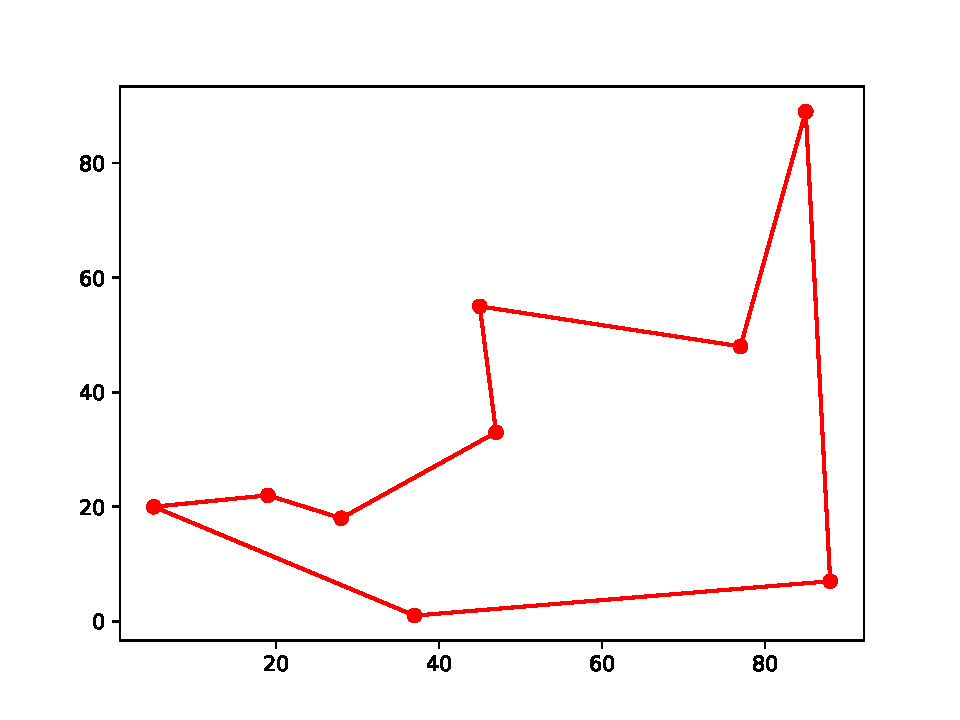
\includegraphics[width=1\textwidth]{pdh.pdf}
  \caption{Problem des Handlungsreisende}
  \label{img:01}
\end{figure}

\section{Fehleranalyse einer gedämpften Schwingun}

%\section*{Quellen}
%\bibliographystyle{plain}
%\bibliography{bibliography}

\listoffigures
%\listoftables

\end{document}